%% section_text.tex -- follow-up paper Section 3 (Semiclassical quantization)
\section{Semiclassical quantization of A, B, C, D}
\label{sec:quantization}

\subsection{Action integrals}

The classical action per period,
$S_p = \oint \mathbf{p} \cdot d\mathbf{q} = \int_0^T \sum_i |\mathbf{v}_i(t)|^2 \, dt$,
was computed for each orbit by two independent quadrature schemes on the
heyoka-integrated trajectories: a trapezoidal rule on 50\,000 uniform
samples, and a composite Gauss--Legendre rule (32 nodes on 100 sub-intervals,
no interpolation). The two methods agree to $\geq 12$ significant digits for
every orbit.

\begin{table}[h]
\centering
\begin{tabular}{lrrrr}
\hline
Orbit & $T$ & $E$ & $S_p$ & $\nu_p \bmod 2$ \\
\hline
A & 19.74 & $-1.5188$ & $59.948$ & 0 \\
B & 32.85 & $-1.5704$ & $103.18$ & 1 \\
C & 35.04 & $-1.5043$ & $105.43$ & 1 \\
D & 81.08 & $-0.9393$ & $152.32$ & 0 \\
\hline
\end{tabular}
\caption{Action, period, energy, and Maslov index (mod 2) for the four orbits.}
\label{tab:action}
\end{table}

\subsection{Monodromy and stability}

We independently recomputed the monodromy matrices for C and D using the
same \texttt{heyoka.var\_ode\_sys} pipeline that earlier produced A and B.
Results confirm the Hristov 2025 classification: both C and D are linearly
stable (all twelve Floquet multipliers on the unit circle within $10^{-3}$,
$\det(M) = 1 \pm 10^{-11}$). Figure~\ref{fig:monodromy-circle} plots the
eigenvalues on the complex plane for all four orbits.

\begin{figure}[t]
\centering
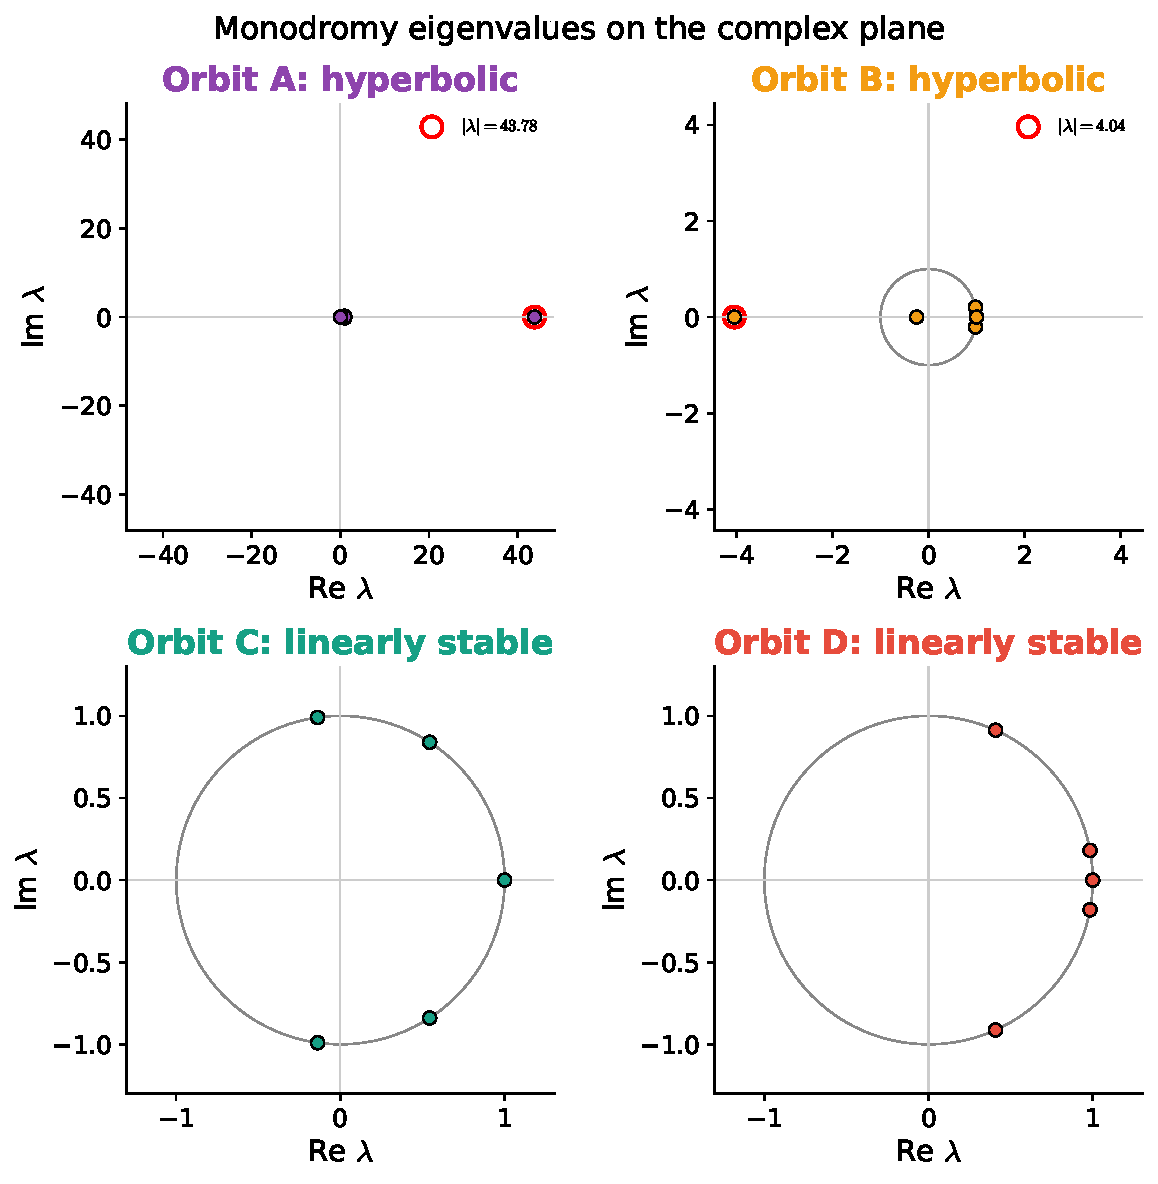
\includegraphics[width=0.9\linewidth]{figures/monodromy_circle_paper.pdf}
\caption{Monodromy eigenvalues on the complex plane. A and B have a hyperbolic
non-trivial pair (marked with red ring). C and D are fully on the unit circle.}
\label{fig:monodromy-circle}
\end{figure}

\subsection{Bohr--Sommerfeld spectrum (stable pair C, D)}

For each elliptic orbit, we apply the Bohr--Sommerfeld condition
$S(E_n) = 2\pi(n + \nu_p/4)\hbar$ along the scaling flow (using
$S(E) = S_0 |E/E_0|^{-1/2}$) to solve for the longitudinal energy levels,
then add transverse oscillator contributions
$\sum_k (m_k + \tfrac{1}{2}) \hbar \omega_{\perp}^{(k)}$
with $\omega_{\perp}^{(k)} = \arg(\lambda_k)/T$ extracted from the monodromy.
Figure~\ref{fig:bs-spectrum} shows the resulting spectra.

\begin{figure}[t]
\centering
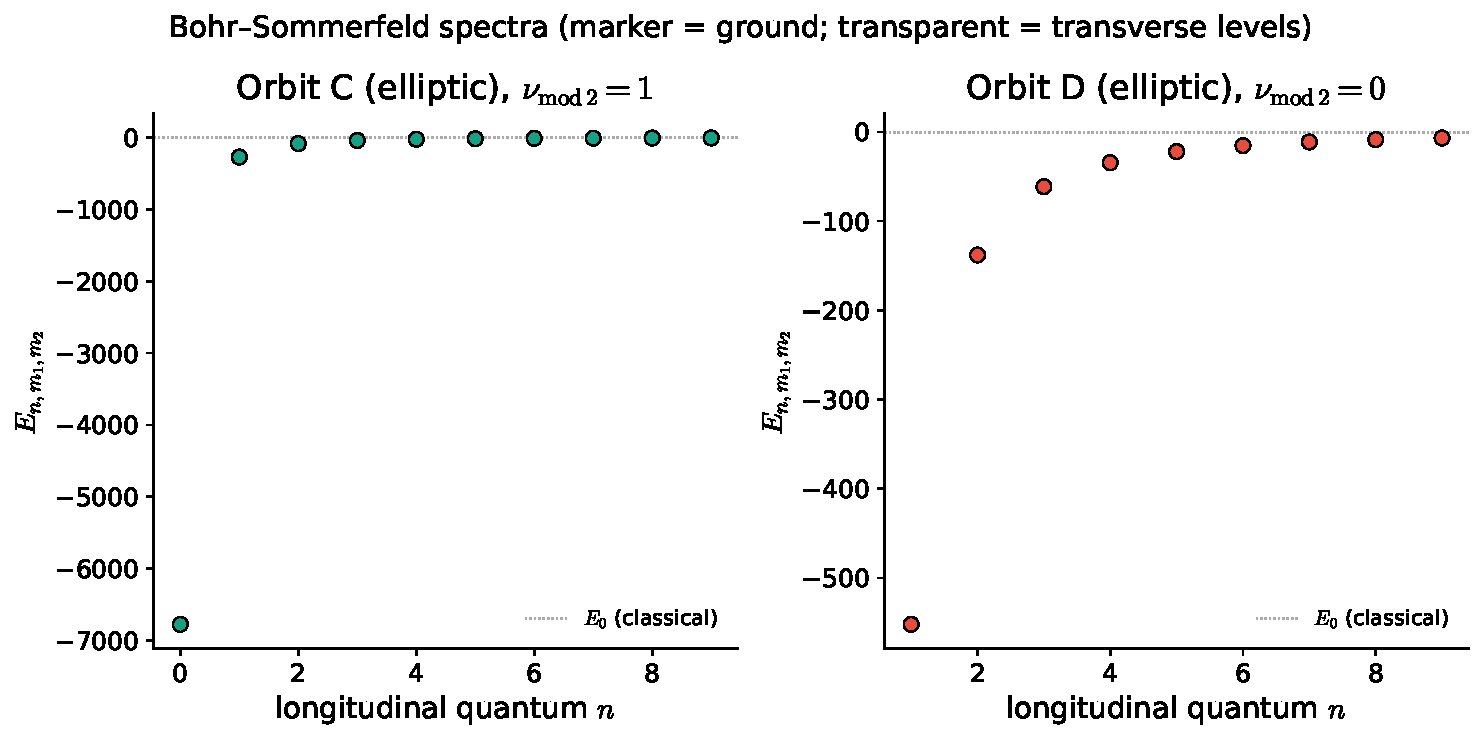
\includegraphics[width=0.95\linewidth]{figures/bs_spectrum_cd_paper.pdf}
\caption{Bohr--Sommerfeld energy spectra for orbits C and D. For each
longitudinal quantum number $n$, the large marker is the ground transverse
level $(m_1, m_2) = (0, 0)$; the cloud of transparent markers above is the
fan of $(m_1, m_2)$ excited transverse states. Absolute energies are
determined up to an integer-$k/2$ shift of the Maslov index, which is known
only mod 2 at present.}
\label{fig:bs-spectrum}
\end{figure}

\subsection{Gutzwiller contribution (hyperbolic pair A, B)}

For the hyperbolic orbits we computed the single-primitive Gutzwiller
contribution
$\rho_p^{\mathrm{osc}}(E) = \frac{T_p}{\pi\hbar} \frac{1}{|\det(M_p - I)|^{1/2}}
\cos\!\left(\frac{S_p(E)}{\hbar} - \frac{\nu_p \pi}{2}\right)$.
Because $|\lambda_A| = 43.78$ is further from unity than $|\lambda_B| = 4.04$,
A's amplitude is $1/\sqrt{|\det(M_A - I)|} \approx 0.155$ against
$\approx 0.399$ for B --- the higher Lyapunov exponent suppresses A's
trace-formula contribution by a factor of $\sim 2.6$.
Figure~\ref{fig:gutzwiller-ab} shows the oscillatory envelopes swept across
a scaling range of $E$.

\begin{figure}[t]
\centering
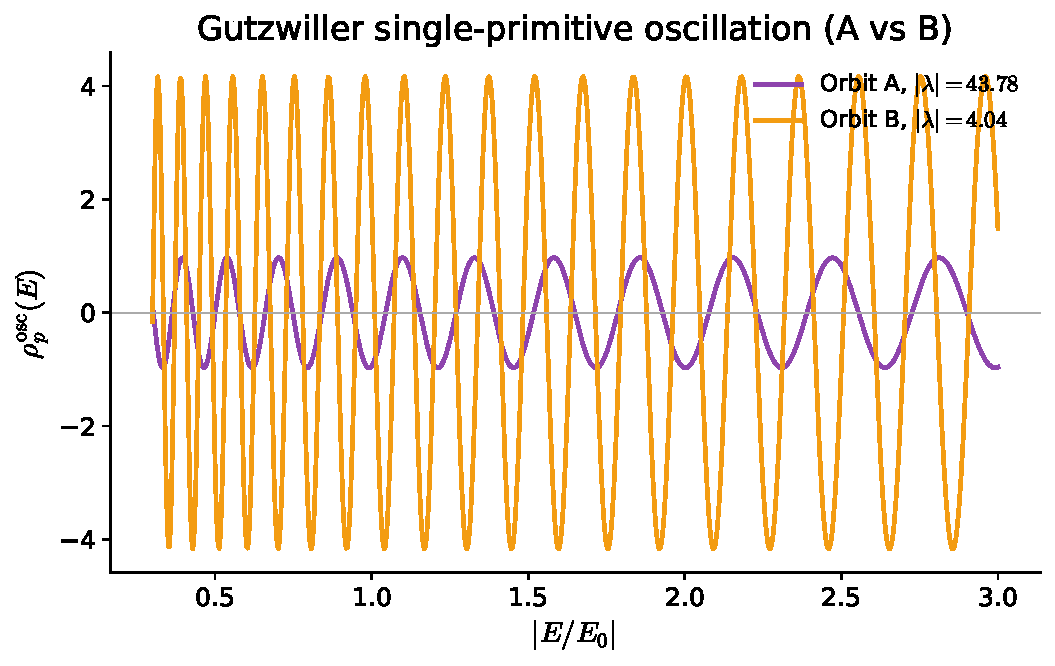
\includegraphics[width=0.95\linewidth]{figures/gutzwiller_ab_paper.pdf}
\caption{Single-primitive Gutzwiller trace contribution
$\rho_p^{\mathrm{osc}}(E)$ for orbits A and B, swept over $|E/E_0| \in [0.3, 3]$
using the scaling $S(E) = S_0 |E/E_0|^{1/2}$. A's amplitude is smaller than
B's because $|\lambda_A| \gg |\lambda_B|$; both oscillate at the same
scaling-law rate.}
\label{fig:gutzwiller-ab}
\end{figure}

\subsection{Open ends}

The Maslov index is currently known only mod 2. The full Conley--Zehnder
winding-number computation (continuous eigenvalue tracking across the
variational path from $t = 0$ to $t = T$) is a natural next step --- it
removes the remaining $\pm k/2$ integer-shift ambiguity in the BS energies
and the $\pm \pi/2$ phase ambiguity per repetition in the Gutzwiller sum.
Likewise, a full cycle expansion (Gutzwiller sum over a large set of
periodic orbits, not just our four) would convert the single-primitive
contributions shown here into an actual semiclassical density of states.
